\documentclass{beamer}

\usepackage[T1]{fontenc}
\usepackage[utf8]{inputenc}
\usepackage[slovene]{babel}
\usepackage{palatino}
\usefonttheme{serif}
\usepackage{amsmath,amssymb,amsfonts, mathtools}
\graphicspath{{./images/}}

\usetheme{CambridgeUS}
\usecolortheme{dolphin}
\setbeamertemplate{navigation symbols}{}

\linespread{1.2}

\newcommand{\N}{\mathbb{N}}
\newcommand{\Z}{\mathbb{Z}}
\newcommand{\Q}{\mathbb{Q}}
\newcommand{\R}{\mathbb{R}}
\newcommand{\C}{\mathbb{C}}

\theoremstyle{definition} % tekst napisan pokoncno
\newtheorem{definicija}{Definicija}[section]
\newtheorem{primer}[definicija]{Primer}
\newtheorem{opomba}[definicija]{Opomba}

\theoremstyle{plain} % tekst napisan posevno
\newtheorem{lema}[definicija]{Lema}
\newtheorem{izrek}[definicija]{Izrek}
\newtheorem{trditev}[definicija]{Trditev}
\newtheorem{posledica}[definicija]{Posledica}

\title[Gramatike za kodiranje podatkov]{Kontekstno-neodvisne gramatike za kodiranje in stiskanje podatkov}
\author{Janez Podlogar}
\institute[UL-FMF]{Univerza v Ljubljani, Fakulteta za matematiko in fiziko}
\date[November 2022]{21. 11. 2022}

\begin{document}

\begin{frame}
    \titlepage
\end{frame}

\section{Kodiranje podatkov}

\begin{frame}{Kodiranje in kod}
    
    Zapis informacije v neki obliki ni primeren za vsakršno rabo. Spreminjanje zapisa sporočila
    pravimo \textit{kodiranje}, sistemu pravil, po katerem se kodiranje opravi, pa \textit{kod}.

\end{frame}

\begin{frame}{Primer kodiranja}

    \textit{Morsejeva abeceda} je kodiranje črk, števil in ločil s pomočjo zaporedja kratkih
    in dolgih signalov:

    \begin{itemize}
        \item Dolžina kratkega signala je ena enota.
        \item Dolgi signal je trikrat daljši od kratkega signala.
        \item Razmik med signali znotraj črke je tišina dolžine kratkega signala.
        \item Razmik med črkami je tišina dolga tri kratke signale oz. en dolgi signal.
        \item Presledek med besedami je tišina dolga sedmih kratkih signalov.
    \end{itemize}

\end{frame}

\begin{frame}{Morsejeva abeceda}

    \begin{figure}[h]
        \centering
        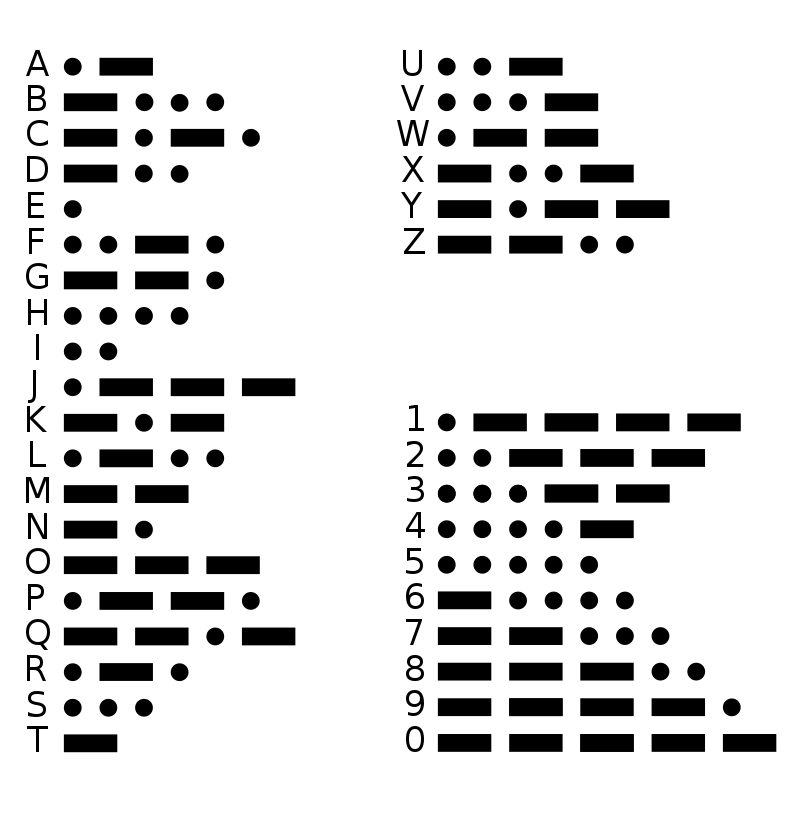
\includegraphics[width=4.3cm]{International_Morse_Code.svg.png}
        \caption{Mednarodna Morsejeva abeceda}
    \end{figure}
    
\end{frame}

\begin{frame}{Abeceda in nizi na abecedi}
    
    \begin{definicija}

        \textit{Abeceda} je končna neprazna množica $ \Sigma $. Elementom abecede pravimo \textit{črke}.
        \textit{Množica vseh končnih nizov abecede} $ \Sigma $ označimo z $ \Sigma^* $ in vključuje tudi
        prazen niz, ki ga označimo z $ \varepsilon $. \textit{Dolžino niza w} označimo z $ |w| $ in je 
        enaka številu črk v nizu $ w \in \Sigma^* $. \textit{Jezik na abecedi} $ \Sigma $ je poljubna
        podmnožica množice $ \Sigma^* $. 
    
    \end{definicija}

    \pause
    
    \begin{primer}

    Naj bo $ \Sigma = \{ a,b,c \} $ abeceda, potem je
    \begin{gather*} 
        ab \in \Sigma^* \\
        cababcccababcccab \in \Sigma^*
    \end{gather*}

    \end{primer}

\end{frame}

\begin{frame}{Kodiranje in dekodiranje}
    
    \begin{definicija}
    
        \textit{Kodiranje nizov abecede} $ \Sigma $ je injektivna funkcija $ \kappa \colon \Sigma^* 
        \to \Sigma_c^* $, kjer je $ \Sigma_c $ \textit{kodirna abeceda} in $ \kappa(w) $ imenujemo
        \textit{koda niza} $ w $. \textit{Dokodiranje kodiranja} $ \kappa $ je funkcija 
        $ \kappa^{-1} \colon C \subseteq \Sigma^*_c \to \Sigma^* $, da velja
        \[
            \forall w \in \Sigma^* \colon \kappa^{-1}(\kappa(w)) = w
        \]
    
    \end{definicija}

\end{frame}

\begin{frame}{Formalizirzacija Morsejeve abecede}

    Abecedi sta
    \begin{gather*}
        \Sigma = \{ \text{A},  \text{B}, \ldots, \text{Z} \} \cup \{ 0, 1, \ldots, 9 \} \cup \{ \_ \} \\
        \Sigma_c = \{ \cdot ,-, \_ \}
    \end{gather*}
    Definirajmo kodno funkcijo črk abecede $ \kappa \colon \Sigma \to \Sigma_c^* $, ki vsakei črki iz abecede
    $ \Sigma $ priredi niz črk kodirne abecede $ \Sigma_c $. Za niz $ w = a_1a_2 \ldots a_n \in \Sigma^* $
    definiramo kodirno funkcijo $ K $ po črkah
    \[
        K(w) = \kappa(a_1)\_\kappa(a_2)\_\cdots\kappa(a_n)
    \]

\end{frame}

\begin{frame}{Formalizirzacija Morsejeve abecede}
    
    Vrednosti funkcije $ \kappa $ so določene s
    tabelo
    \begin{figure}[h]
        \centering
        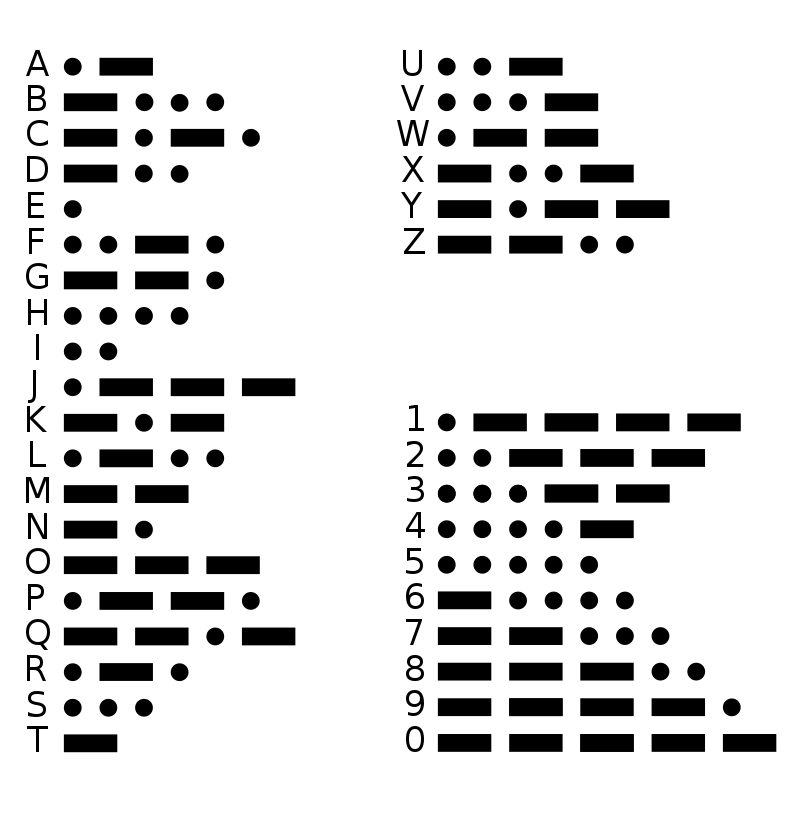
\includegraphics[width=3cm]{International_Morse_Code.svg.png}
    \end{figure}
    Dodatno presledek med besedami \_  kodiramo v sedem kratkih enot tišine 
    \[
        \kappa(\_) = \_\_\_
    \]

\end{frame}

\section*{Stiskanje podatkov}

\begin{frame}{Stiskanje podatkov}
    
    \begin{definicija}
    
        \textit{Stiskanje} je kodiranje $ K $ za katerega velja 
        \[ 
        \exists n \in \N \ \forall w \in \Sigma^* \colon |w| \geq n \implies
        \left\lvert K(w)\right\rvert \ll \left\lvert w \right\rvert
        \]
    
    \end{definicija}

\end{frame}

\begin{frame}{Zgled stiskanja niza $ w $}

    Za abecedo vzemimo $ \Sigma = \{ a,b,c \} $ in poglejmo niz
    \[
        w = cababcccababcccab
    \]
    \pause
    Uvedemo novi spremenljivki $ A = ab $ in $ B = ccc $.
    \[
        w = cAABAABA
    \]
    \pause
    Uvedemo novo spremeljivko $ C = AAB $.    
    \[
        w = cCCA
    \]

\end{frame}

\begin{frame}{Zgled stiskanja niza $ w $}
    
    Prešnji postopek napišemo na sledeč način s pomočjo produkcijskih pravil
    \begin{align*}
        & S  \rightarrow  cCCA, \\
        & A  \rightarrow  ab, \\
        & B  \rightarrow  ccc, \\
        & C  \rightarrow  AAB
    \end{align*}

\end{frame}

\section*{Kontekstno-neodvisne gramatike}

\begin{frame}{Kontekstno-neodvisne gramatike}
    
    \begin{definicija}

        \textit{Formalna gramatika} $ G $ so pravila, ki nam iz abecede $ \Sigma $ tvorijo jezik,
        označimo ga z $ L(G) $
    
    \end{definicija}
    
    \pause

    \begin{definicija}
    
        \textit{Kontektsno-neodvisna gramatika} je četverica $ G = ( V, \Sigma, P, S ) $, kjer je
        $ V $ končna množica \textit{spremenljivk}, abeceda $ \Sigma $ množica \textit{končnih simbolov} tako,
        da $ \Sigma \cap V = \emptyset $, $ P \subseteq V \times ( V \cup \Sigma )^* $ relacija, ki ji
        pravimo \textit{produkcijsko pravilo} in $ S \in V $ \textit{začetna spremenljivka}.
    
    \end{definicija}

\end{frame}

\begin{frame}{Kontekstno-neodvisne gramatike}
    
    \begin{definicija}
    
        Naj bo $ G = ( V, \Sigma, P, S ) $ kontekstno-neodvisna gramatika. Naj bodo $ \alpha $,
        $ \beta $, $ \gamma \in ( V \cup \Sigma )^* $ nizi spremenljivk in končnih simbolov,
        $ A \in V $ spremenljivka ter naj bo $ ( A, \beta ) \in P $ produkcijsko pravilo,
        označimo ga z $ A \rightarrow \beta $. Pravimo, da se $ \alpha A \gamma $ 
        \textit{prepiše s pravilom} $ A $ v $ \alpha\beta\gamma $, pišemo $ \alpha A \gamma  \Rightarrow 
        \alpha\beta\gamma $. Pravimo, da $ \alpha $ \textit{porodi} $ \beta $, če je $ \alpha = \beta $ ali če
        za $ k \geq 0 $ obstaja zaporedje $ \alpha_1, \alpha_2, \ldots \alpha_n
        \in ( V \cup \Sigma )^* $ tako, da 
        \[
            \alpha \Rightarrow \alpha_1 \Rightarrow \alpha_2 \Rightarrow \ldots \Rightarrow \alpha_n
            \Rightarrow \beta
        \]
        in pišemo $ \alpha \xRightarrow{*} \beta $.
    
    \end{definicija}

\end{frame}

\begin{frame}{Kontekstno-neodvisne gramatike}
    
    \begin{posledica}
    
        Jezik kontekstno neodvisne gramatike $ G $ je
        \[
            L(G) = \{ w \in \Sigma^* \mid S \xRightarrow{*} w \}
        \]
    
    \end{posledica}

\end{frame}

\begin{frame}{Zgled stiskanja niza $ w $ z zapisom gramatike}
    
    Formalizirajmo gramatiko iz prejšnjega primera. Gramatiko smo generirali z nizom
    $ w = cababcccababcccab $.
    \pause
    Označimo jo z $ G_w = ( V, \Sigma, P, S ) $, kjer je 
    \begin{gather*}
        V = \{ S, A, B, C \}, \\
        \Sigma = \{ a, b, c \}, \\
        P = \{ S  \rightarrow  cCCA, A  \rightarrow  ab, B  
        \rightarrow  ccc, C  \rightarrow  AAB \}, \\
        S = S
    \end{gather*}
    \pause
    Vidimo, da $ G_w $ ustreza naši definiciji kontekstno-neodvisne gramatike
    in res kodira $ w $, saj je 
    \[
        L(G_w) = \{w\}
    \]

\end{frame}

\end{document}